\section{Task 2: Building a vision-language model and testing whether it looks}
\label{sec:task2}

The vision-language model passes SigLIP-base patch features (196 per image) through a two-layer MLP connector, scaled by $s=0.055$ to match the norm of text embeddings, into Qwen3-0.6B's prompt before the question, as in LLaVA~\citep{liu2023llava}. A single run of 4,500 updates moves through three stages: COCO captions with only the connector training (2,250 updates), generated presence and counting questions with rank-16 LoRA added (1,500), and natural VQAv2 questions (750), each stage replaying earlier data. The test uses held-out complementary pairs~\citep{goyal2017vqav2}: an annotation-derived suite of presence and counting questions (64 pairs) and a natural VQAv2 suite (96 pairs). Every question is answered greedily four times, with the correct image, the partner image, an unrelated image and no image, so the answers can be compared across inputs while the question stays fixed.

\begin{table}[t]
  \centering
  \small
  \setlength{\tabcolsep}{4pt}
  \begin{tabular}{llccccc}
    \toprule
    Suite & Image input & accuracy (\%) & pair acc. & identical & partner match & ref. NLL \\
    \midrule
    \multirow{4}{*}{\shortstack[l]{Grounding\\(64 pairs)}}
      & correct       & 68.8 \ci{59.4}{78.1} & 54.7 & 15.6 & 14.1 & 1.0 \\
      & complementary & 14.1 \ci{8.6}{19.5}  & 0.0  & 15.6 & 68.8 & 3.5 \\
      & mismatched    & 42.2 \ci{35.9}{48.4} & 6.2  & 81.3 & 35.9 & 2.2 \\
      & none          & 0.0                  & 0.0  & 100  & 0.0  & 8.0 \\
    \midrule
    \multirow{4}{*}{\shortstack[l]{VQAv2\\(96 pairs)}}
      & correct       & 55.6 \ci{47.9}{63.1} & 32.3 & 39.6 & 17.7 & 1.5 \\
      & complementary & 21.8 \ci{16.4}{27.3} & 1.0  & 39.6 & 53.1 & 3.0 \\
      & mismatched    & 28.3 \ci{22.6}{34.0} & 2.1  & 61.5 & 29.7 & 2.8 \\
      & none          & 0.0                  & 0.0  & 100  & 0.0  & 10.0 \\
    \bottomrule
  \end{tabular}
  \caption{\textbf{Task 2 final test} (196 visual tokens, greedy decoding, original references throughout; rates in \%). Pair acc.: both questions of a pair right. Identical: both receive the same answer. Partner match: answer equals the partner image's answer. Correct-image advantage over the swap: grounding $+54.7$\pp\ci{40.6}{68.0} in accuracy and $+2.5$ nats\ci{1.9}{3.0} in NLL; VQAv2 $+33.9$\pp\ci{24.3}{43.4} and $+1.5$\ci{1.1}{2.0}. No answer was empty. Source: \file{final\_*\_test.csv}, \file{advantages.csv}.}
  \label{tab:task2}
\end{table}

With the correct image the model answers 68.8\% of grounding questions and 55.6\% of VQAv2 questions correctly (Table~\ref{tab:task2}). With the partner image, accuracy against the original reference drops to 14.1\% and 21.8\%, and the reference answer becomes 2.5 and 1.5 nats less likely, both advantages well clear of zero. The swap row needs careful reading. Under greedy decoding, the swapped input of one question is exactly the correct input of the other, since both share the question and differ only in the image. The row therefore repeats the same answers scored against the other reference, and the informative quantity is how often the two images of a pair receive different answers, which would never happen for a model that ignores the image. Here it happens in 84.4\% of grounding pairs and 60.4\% of VQAv2 pairs, with both answers right in 54.7\% and 32.3\%. When the image changes, the answer mostly moves to what the new image supports (68.8\% and 53.1\% partner match); only 17.2\% and 29.2\% of swapped answers match neither image.

The other two controls show where the answers come from. An unrelated image rarely contains the asked object, so the model's ``no'' is often correct: presence accuracy reaches 53.1\% with an unrelated image against 7.8\% with the partner image, and VQAv2 yes/no reaches 56.8\%, while for counting, number and other questions the two conditions overlap. Answers to unrelated images are also more uniform (81.3\% identical within grounding pairs), consistent with a default answer when nothing relevant is visible. Without any image the score is 0\%, but this does not mean the model has no prior. Without visual tokens it answers in full sentences (``No, the image does not contain a toilet.''), and 98 to 100\% of these answers have more than three words, so exact match fails. The short-answer format was learned only with visual tokens present, and an input without them never occurred in training. The prior is better read from the likelihoods, under which the reference answer is 7 to 8.5 nats less likely than with the image. The sentences also make generation slower without an image, despite a prompt 196 tokens shorter.

Accuracy differs strongly by question type (Figure~\ref{fig:task2types} and Table~\ref{tab:task2ex} in the appendix). Presence is nearly solved (92.2\%) and the swap almost always flips it. Every type beats the best constant answer, but counting (45.3\% against 28.1\%) and VQAv2 number questions (49.2\% against 29.2\%) remain hard, and with 32 and 24 pairs their intervals span about 25 points. The annotation-derived suite is answered more accurately and more image-dependently (swap advantage 54.7 against 33.9 points), as its cleaner labels would predict: a ``no'' requires that no instance of the object is annotated, and counts are asked only when every instance is unambiguous. The first pair of each type in the seeded test order, a rule fixed before any output was seen, shows these patterns. Presence and yes/no pairs are the clean case, with both answers right and both flipped by the swap. The counting pair receives ``2'' for both images, and the ``other'' pair receives ``traffic'' for both images where the references are ``sun'' and ``rain'', an answer tied to the scene but blind to the difference between the images.

\begin{figure}[t]
  \centering
  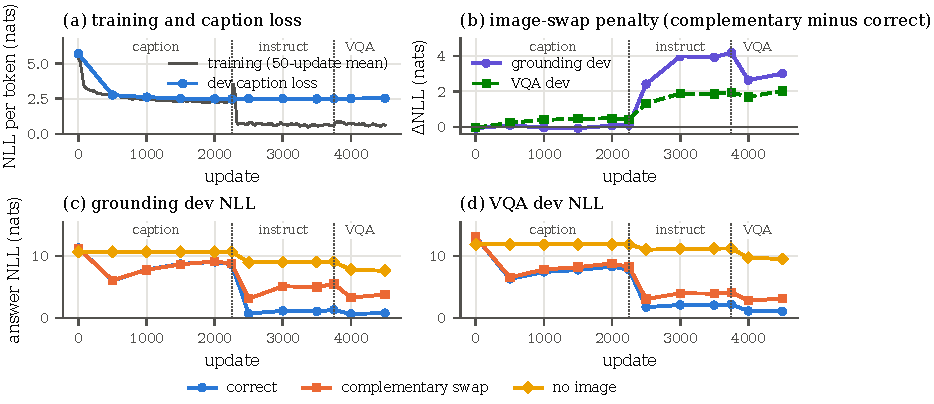
\includegraphics[width=\linewidth]{fig_task2_curves.pdf}
  \caption{\textbf{Task 2 learning curves}, with stage boundaries dotted. (a) Training loss (50-update mean; its mixture changes at each boundary) and development caption loss (96 images). (b) Image-swap penalty $\Delta$NLL on the development suites (24 grounding and 32 VQAv2 pairs). (c, d) Reference-answer NLL under the correct image, the partner image and no image. Source: \file{dev\_metrics.csv}.}
  \label{fig:task2curves}
\end{figure}

The development curves show how this image dependence emerged (Figure~\ref{fig:task2curves}). Besides losses, they track the image-swap penalty $\Delta\mathrm{NLL}=\mathrm{NLL}(y\mid q,I_{\mathrm{partner}})-\mathrm{NLL}(y\mid q,I_{\mathrm{correct}})$, which is positive when the correct image makes the reference answer $y$ more likely. Caption alignment works quickly: development caption loss falls from 5.69 to 2.76 nats within 500 updates and ends the stage at 2.48. Short-answer NLL first falls with it (grounding 11.3 to 6.0, VQAv2 13.1 to 6.3) as the visual tokens become usable input, then rises again for the rest of the stage, to as much as 9.0 and 8.3, apparently because training on one-sentence descriptions makes a bare ``yes'' or ``2'' less likely. In this stage the grounding swap penalty stays between $-0.07$ and $0.11$ nats, while the VQAv2 penalty grows to 0.49 without a single VQA question: caption training alone makes natural answers such as colours, sports or objects somewhat image-dependent, but not the templated ones. The instruct stage then does most of the work for both suites. Within 250 updates, grounding NLL under the correct image falls to 0.69 and its swap penalty jumps to 2.41 (peaking at 4.19), and VQAv2 NLL drops from 7.8 to 1.7 although this stage contains no VQAv2 question. The VQA stage lowers VQAv2 NLL further (2.2 to 1.1) and ends with a swap penalty of 2.03, while replay keeps caption loss near 2.5 throughout. The no-image NLL is constant through stage 1, as it must be when only the connector trains, and falls once LoRA trains (to 7.60 and 9.51): the adapters learn some answer prior that needs no image, yet it stays 6.8 to 8.4 nats above the correct-image value.

Compressing the visual input changes little. The optional 49-token run, which averages each $2\times2$ block of patches before a fresh connector, leaves grounding unchanged (68.0\% against 68.8\%) and lowers VQAv2 accuracy (52.8\% against 55.6\%) and its swap advantage (26.6 against 33.9 points), all within overlapping intervals. It trains in 8.3 instead of 13.3 minutes at almost the same peak memory (4.33 against 4.48\,GiB), most of which is the cached feature bank. The whole 196-token pipeline is cheap: 2.5 minutes of feature caching, 13.3 minutes of training, 6.42M trainable parameters and 21\,s of final evaluation.
